\documentclass[journal]{IEEEtran}

\usepackage[utf8]{inputenc}
\usepackage[T1]{fontenc}
\usepackage{lmodern}
\usepackage{xcolor}
\usepackage{pgfplots}
\pgfplotsset{compat=1.17}
\usepackage{amsmath,amssymb,amsthm}
\usepackage{booktabs}
\usepackage{enumitem}
\usepackage{tikz}
\usetikzlibrary{arrows.meta, positioning, calc, fit, backgrounds}
\usepackage[hidelinks]{hyperref}
\usepackage{url}

\definecolor{valen}{RGB}{30,90,170}
\definecolor{valenred}{RGB}{190,50,50}
\definecolor{valengreen}{RGB}{30,130,70}

\newcommand{\R}{\mathbb{R}}
\newcommand{\N}{\mathbb{N}}
\newcommand{\valen}{\textsc{Valen}}
\newcommand{\IR}{\mathcal{G}}

\newtheorem{definition}{Definición}
\newtheorem{theorem}{Teorema}
\newtheorem{proposition}{Proposición}
\newtheorem{lemma}{Lema}
\newtheorem{corollary}{Corolario}

\title{Invariantes Estructurales y Matemática de Grafos de Ataque:\\ Una Plataforma Ofensiva--Defensiva Autónoma}

\author{Proyecto \valen}

\begin{document}
\maketitle

\begin{abstract}
Presentamos \valen\ (\emph{Verification And Active Logic Engine, Neuro-symbolic}),
un sistema integral que une una tesis \emph{defensiva} medida con una plataforma
\emph{ofensiva} sobre una única representación intermedia en grafo tipado
($\IR$). En lo defensivo, zanjamos una pregunta de frontera con rigor estadístico:
los invariantes espectrales, de homología (persistente y dirigida) y de curvatura
discreta de los grafos de programa no aportan \emph{información} más allá del
taint para priorizar inyecciones (OWASP Benchmark~1.2, $2740$ casos; taint MRR
$0.894$, AUC $0.895$, campo fusionado $0.872$, permutación pareada
$p=5\times10^{-5}$), aunque son la \emph{única} señal para autorización
(BOLA/IDOR: recall $1.0$ / precisión $0.90$ en crAPI), ciclos destructivos de
estado (homología dirigida GLMY: $0.97$ vs.\ $0.065$ de recall frente a la
simetrizada) y topología de confianza. En lo ofensivo, \valen\ es una plataforma
de red teaming autónoma --- un servidor multi-usuario que coordina reconocimiento,
análisis de grafos de Active Directory, comando y control, recuperación de
credenciales, phishing y exfiltración --- cuyo diferencial es una
\emph{matemática de grafos de ataque} que enunciamos y probamos: cortes mínimos de
Menger (puntos de estrangulamiento), flujo de costo mínimo, probabilidades de
impacto de cadenas de Markov absorbentes resueltas exactamente por
$(I-Q)^{-1}R$, síntesis de planes de explotación de costo mínimo mediante
bounded model checking con Z3-Optimize (con precondiciones AND), y una gramática
libre de contexto probabilística para adivinar contraseñas. El agente resuelve
$18/18$ retos documentados de crAPI de forma autónoma (incluidos tres retos de
inyección de prompt sobre un LLM).
\end{abstract}

\begin{IEEEkeywords}
invariantes estructurales, análisis de taint, topología dirigida, grafos de
ataque, red teaming autónomo, síntesis formal, adivinación de contraseñas
\end{IEEEkeywords}

\section{Introducción}
\IEEEPARstart{D}{os} preguntas organizan este trabajo. \emph{Primera, ¿dónde
aportan los invariantes estructurales de los grafos de programa información de
seguridad, y dónde no?} \emph{Segunda, ¿puede la misma maquinaria convertirse en
un motor de planificación cuantitativa para operaciones ofensivas?} La respuesta a
la primera es una frontera nítida y estadísticamente zanjada
(\S\ref{sec:boundary}); la respuesta a la segunda es una plataforma operativa cuyo
diferencial es la matemática, no el scripting (\S\ref{sec:platform},
\S\ref{sec:math}).

Nuestras contribuciones son:
\begin{enumerate}[label=\textbf{C\arabic*.},leftmargin=2.2em]
\item Una \emph{frontera medida} sobre los priors geométricos para SAST de
  inyección, con test de permutación pareado e intervalos de confianza bootstrap.
\item Un \emph{invariante de autorización operativo} mecanizado en Lean~4, un
  detector estructural de BOLA/IDOR y un testigo Z3 de propiedad que separa la
  autorización a nivel de objeto de la autenticación.
\item Evidencia de que la \emph{homología dirigida GLMY} es la señal correcta de
  ciclos, dominando a la homología simetrizada.
\item Una \emph{frontera de arbitraje neuro-simbólico} medida: el LLM propone, los
  métodos formales disponen.
\item Un \emph{front-end SAST multi-lenguaje}: un motor de taint genérico que
  conduce nueve gramáticas.
\item Una \emph{plataforma de red teaming autónoma} con un modelo de autorización
  primero.
\item \emph{Matemática de grafos de ataque} con pruebas: chokepoints, planes de
  costo mínimo y disjuntos, probabilidades de impacto exactas, síntesis de
  explotación de costo mínimo y un prior PCFG de contraseñas.
\end{enumerate}

\section{Marco formal}
\label{sec:framework}

\begin{definition}[IR tipado]
\label{def:ir}
Un \emph{grafo tipado} es un multigrafo dirigido
$\IR=(V,E,\tau_V,\tau_E,\alpha)$ donde $\tau_V:V\to\mathcal{K}_V$ etiqueta los
vértices (módulo, función, sumidero, compuerta, principal, \dots),
$\tau_E:E\to\mathcal{K}_E$ etiqueta las aristas (control, dato, llamada, taint,
confianza, autenticación, \dots), y $\alpha:E\to\Sigma^{*}$ asocia atributos como
un nombre de relación o un costo. Cada adaptador emite el mismo $\IR$, de modo que
todas las capas de análisis son agnósticas al motor.
\end{definition}

\begin{definition}[Campo estructural]
\label{def:field}
Un \emph{campo estructural} es una función $V(x):\IR\to\R^{d}$ que fusiona las
señales algebraica (retículo de taint, nivel de privilegio), espectral (vector de
Fiedler), topológica ($H_0,H_1$ persistentes y $H_1$ dirigida GLMY) y geométrica
(curvatura de Forman--Ollivier Ricci) en una puntuación por nodo usada para
priorizar.
\end{definition}

\begin{definition}[Retículo de privilegios y arista de autenticación]
\label{def:auth}
Sea $F:V\to\N$ un nivel de privilegio. Una arista $e=(u,v)$ con
$\tau_E(e)=\texttt{auth}$ es una \emph{arista de autenticación} si $F(u)<F(v)$. Un
camino $\pi=v_0\to\cdots\to v_k$ es \emph{no vigilado} (ungated) si ninguna de sus
aristas es de autenticación.
\end{definition}

\begin{proposition}[Sin escalada de privilegios sin aristas de autenticación]
\label{prop:auth}
Si $\pi=v_0\to\cdots\to v_k$ no está vigilado, entonces $F(v_k)\le F(v_0)$.
\end{proposition}
\begin{proof}
Toda arista no autenticada es intra-nivel o \emph{descendente} en el retículo, es
decir, para cada arista $e=(v_i,v_{i+1})$ de $\pi$ se cumple $F(v_{i+1})\le
F(v_i)$. Por transitividad $F(v_k)\le F(v_0)$. El enunciado está mecanizado en
Lean~4 como \texttt{no\_auth\_bounded}; la solidez de la abstracción booleana de
taint es \texttt{prop1\_soundness}. \qedhere
\end{proof}

\begin{definition}[Grafo de ataque y costo]
\label{def:cost}
Un \emph{grafo de ataque} es un $\IR$ cuyos vértices son principales y cuyas
aristas $m\to n$ son \emph{acciones} que requieren el control de $m$ y producen el
control de $n$. Un \emph{modelo de costo} es $c:E\to\R_{>0}$ (sigilo más esfuerzo;
p.\ ej.\ $c(\mathrm{MemberOf})=1$, $c(\mathrm{DCSync})=5$). Dado el conjunto de
entrada $S$ y el objetivo $T$, un \emph{plan de ataque} es un conjunto de aristas
cuyo cierre transitivo conecta algún $s\in S$ con algún $t\in T$.
\end{definition}

\begin{definition}[Probabilidad de impacto]
\label{def:hit}
Para un conjunto objetivo $T\subseteq V$, la \emph{probabilidad de impacto}
$h:V\to[0,1]$ es
\[
h(u)=
\begin{cases}
1 & u\in T,\\
\frac{1}{\deg^{+}(u)}\sum_{v:\,u\to v}h(v) & u\notin T,
\end{cases}
\]
la medida armónica de $T$ bajo un paseo aleatorio uniforme sobre el grafo
dirigido.
\end{definition}

\begin{proposition}[La probabilidad de impacto es la única solución armónica]
\label{prop:hit}
Para los nodos transitorios $u\notin T$, el vector $h_T$ satisface $(I-Q)h_T=r$
donde $Q$ es la matriz de transición transitorio-a-transitorio y
$r_u=\sum_{v\in T}P_{uv}$; la solución es única y puede obtenerse por iteración de
valor o por eliminación gaussiana en $O(|V|^3)$.
\end{proposition}
\begin{proof}
Particionamos $V=T\uplus U$ (transitorio $U$). La ecuación de Bellman es
$h_T=Qh_T+r$ con $Q$ subestocástica (sumas de fila $\le1$, y $<1$ para todo nodo
con un vecino objetivo). Por tanto $I-Q$ es una $M$-matriz, luego no singular, y el
punto fijo es único. La iteración de valor converge porque $Q$ es una contracción
en el subespacio transitorio. \qedhere
\end{proof}

\section{Verificación estructural}
\label{sec:verification}

\subsection{La frontera de los priors geométricos}
\label{sec:boundary}
Sobre OWASP Benchmark~1.2 \cite{owasp2015} ($2740$ casos con verdad de referencia
conocida) un oráculo de priorización ordena todos los candidatos a sumidero y mide
MRR, R@1, NDCG@$k$, más un test de permutación pareado e intervalos de confianza
bootstrap.

\begin{theorem}[Frontera, empírica]
\label{thm:boundary}
Para fallas de inyección lineal, las señales geométricas/espectrales/topológicas
no aportan información de priorización más allá del taint: el taint crudo logra MRR
$0.894$ (AUC $0.895$); el campo estructural fusionado logra $0.872$
($p=5\times10^{-5}$, IC 95\% $[+0.0157,+0.0294]$); espectral ($0.496$) y
topológica ($0.500$) están en el azar y la curvatura por debajo ($0.376$).
\end{theorem}

Es un \emph{resultado negativo publicable}: un servlet plano y casi acíclico no
tiene curvatura ni topología persistente que explotar, y el taint ya es
casi-óptimo allí. La Figura~\ref{fig:boundary} muestra el AUC por señal.

\begin{figure}[!t]
\centering
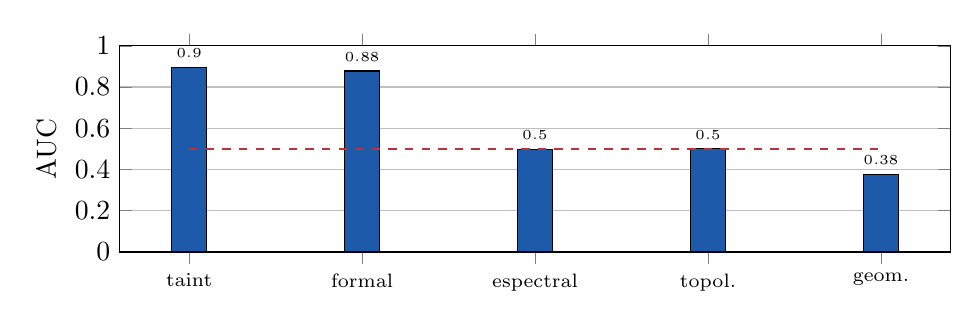
\begin{tikzpicture}
  \begin{axis}[
      ybar, bar width=0.45cm, width=\columnwidth, height=4.2cm,
      symbolic x coords={taint, formal, espectral, topol., geom.},
      xtick=data, x tick label style={font=\scriptsize},
      ymin=0, ymax=1.0, ylabel={AUC},
      nodes near coords, every node near coord/.append style={font=\tiny},
      ymajorgrids=true]
    \addplot[fill=valen] coordinates {
      (taint,0.895) (formal,0.878) (espectral,0.496)
      (topol.,0.500) (geom.,0.376)};
    \draw[dashed, valenred, thick] (axis cs:taint,0.5) -- (axis cs:geom.,0.5);
  \end{axis}
\end{tikzpicture}
\caption{La frontera: espectral y topológica en el azar, curvatura por debajo; el
taint es la señal dominante.}
\label{fig:boundary}
\end{figure}

\subsection{Autorización, mecanizada y operativa}
\label{sec:authz}
La Proposición~\ref{prop:auth} se operativiza en tres artefactos. (i) El detector
estructural de \emph{autorización ausente/BOLA} marca una función con fuente HTTP y
sumidero de recurso sin compuerta de autenticación; sobre un corpus curado de 39
casos alcanza recall $1.0$ / precisión $0.72$ / F1 $0.837$ donde el taint puntúa
$0$. (ii) El verificador Z3 \cite{z3} comprueba
$\mathrm{SAT}(\mathrm{owner}(id)\neq session)$ --- un testigo de propiedad que
separa la autorización a nivel de objeto de la mera autenticación. (iii) En crAPI
($44$ operaciones, $9$ endpoints BOLA/BFLA documentados) una señal de referencia a
objeto recupera los $9$ (recall $1.0$, precisión $0.90$).

\subsection{Homología dirigida}
\label{sec:glmy}
Simetrizar un grafo dirigido es pérdida en ambos sentidos: un $2$-ciclo
$A\to B\to A$ colapsa a una arista no dirigida (una reentrancia perdida) y un
triángulo relleno se vuelve un falso ciclo.

\begin{proposition}[Homología dirigida vs.\ simetrizada]
\label{prop:glmy}
La homología dirigida GLMY $H_1$ \cite{glmy2012} es un superconjunto estricto de la
simetrizada para detectar ciclos destructivos: recall $1.0$ / precisión $0.75$
sobre un corpus de 12 grafos de estado (vs.\ $0.5$/$0.5$) y $0.968$ vs.\ $0.065$
sobre contratos inteligentes curados de SmartBugs.
\end{proposition}

\subsection{Arbitraje neuro-simbólico}
\label{sec:neuro}
Sobre un corpus de 38 archivos ($29$ hallazgos confirmados) la heurística offline
y el agente LiteLLM coinciden en detección y ranking en $37/38$ archivos (acuerdo
$0.974$), mientras el LLM cambia el CWE en $28\%$ de los hallazgos.

\section{SAST multi-lenguaje}
\label{sec:langs}
Un motor de taint genérico conduce nueve gramáticas tree-sitter (C, C++, Rust,
C\#, Go, PHP, Ruby, JavaScript/TypeScript) con perfiles por lenguaje que declaran
fuentes, sumideros, sanitizadores y compuertas de autenticación; Python, Java
(interprocedural) y Solidity tienen adaptadores dedicados.

\section{La plataforma de red teaming}
\label{sec:platform}
\valen\ es un paquete instalable cuyo servidor es un \emph{servidor de equipo}
multi-usuario: usuarios con roles (\texttt{viewer}/\texttt{operator}/
\texttt{admin}), sesiones PBKDF2, RBAC por ruta, compromisos con membresía,
artefactos de evidencia y Server-Sent Events para colaboración en vivo. La
superficie recorre la cadena de destrucción (kill chain) y está limitada por una
lista de alcance, una lista de ejecución (\texttt{--allow-exec}) y la aprobación
del operador.

\section{Matemática de grafos de ataque}
\label{sec:math}

\subsection{Chokepoints vía corte mínimo de Menger}
\begin{theorem}[Menger, forma vértice]
\label{thm:menger}
El número máximo de caminos internamente disjuntos de $S$ a $T$ es igual al número
mínimo de vértices cuya remoción separa $S$ de $T$ \cite{menger1927}.
\end{theorem}
\begin{proof}[Construcción]
Dividimos cada $v$ en $v_{\mathrm{in}}\to v_{\mathrm{out}}$ de capacidad $1$
(ilimitada para $v\in S\cup T$), reemplazamos cada $u\to v$ por
$u_{\mathrm{out}}\to v_{\mathrm{in}}$ de capacidad $\infty$, y añadimos una
super-fuente a $S$ y $T$ a un super-sumidero. Un flujo máximo satura las aristas de
división unitarias de un corte mínimo de vértices (Ford--Fulkerson
\cite{ford1956}). \qedhere
\end{proof}

\subsection{Flujo de costo mínimo}
Enviar $k$ unidades de flujo a costo mínimo, con vértices internos de capacidad
$1$, produce las $k$ rutas de ataque \emph{más baratas y disjuntas}. Implementamos
caminos de aumento sucesivos de costo mínimo (Bellman--Ford sobre el grafo
residual).

\subsection{Probabilidad de impacto}
La Proposición~\ref{prop:hit} da el ranking de riesgo probabilístico; en el corpus
de juguete una entrada con tres aristas salientes y una ruta al objetivo puntúa
$\tfrac13$, una entrada directa $1$.

\subsection{Síntesis formal: planes de explotación de costo mínimo}
\begin{theorem}[Solidez y optimalidad de la síntesis]
\label{thm:synth}
Sea el sistema de transición
\[
\mathrm{has}(s{+}1,n)\equiv \mathrm{has}(s,n)
\vee \bigvee_{e:\,m\to n}\bigl(\mathrm{taken}_e\wedge\mathrm{has}(s,m)\bigr),
\]
con entradas en el paso $0$. Una asignación satisfacible de
\texttt{z3.Optimize} \cite{z3} que minimiza $\sum_e \mathrm{taken}_e\,c(e)$ bajo
$\bigvee_{s\le k}\mathrm{has}(s,t)$ es (i) un plan factible y (ii) de costo mínimo
entre los planes de longitud $\le k$.
\end{theorem}
\begin{proof}
(i) Se sigue por inducción sobre el índice de paso: \texttt{has} es monótona y cada
arista \texttt{taken} tiene su fuente verdadera en el paso en que se dispara. (ii)
El objetivo es exactamente el costo del plan y el optimizador devuelve un mínimo
sobre el espacio de búsqueda acotado. Las acciones compuestas
$\{\mathrm{sources}\to \mathrm{target}\}$ añaden $\bigwedge_{s}\mathrm{has}(s)$
como precondición AND, p.\ ej.\ DCSync requiere Domain Admins \emph{y} una sesión
en un Domain Controller. \qedhere
\end{proof}

\subsection{Adivinación de contraseñas: PCFG}
\begin{definition}[PCFG]
\label{def:pcfg}
Tokenizamos una contraseña en tramos de letras $L$, dígitos $D$, símbolos $S$. Una
\emph{estructura base} es la secuencia de pares $(clase,longitud)$ (p.\ ej.\
$L_6D_4S_1$); los terminales se indexan por $(clase,longitud)$. La probabilidad de
una adivinanza $\sigma$ es
$P(\sigma)=P(\mathrm{structure})\cdot\prod_{t\in\sigma}P(t)$ \cite{weir2009}.
\end{definition}
\begin{proposition}[Enumeración monótona]
\label{prop:pcfg}
La expansión best-first sobre los terminales por ranura, ordenada por probabilidad
decreciente, enumera adivinanzas en $P(\sigma)$ no creciente y sin duplicados.
\end{proposition}
\begin{proof}
La log-probabilidad negativa $-\log P(\sigma)$ es un costo aditivo no negativo por
ranura, de modo que Dijkstra sobre el retículo producto visita las adivinanzas en
costo no decreciente; el conjunto \emph{seen} evita la re-expansión. \qedhere
\end{proof}

\section{Evaluación}
\label{sec:eval}

\subsection{Pentest autónomo contra OWASP crAPI}
Contra un laboratorio crAPI 1.1.5 fresco el agente autónomo resuelve
\textbf{18/18} retos documentados --- BOLA/BFLA, asignación masiva, SSRF, inyección
NoSQL/SQL, falsificación JWT, reseteo de contraseña, límite de tasa y tres retos de
inyección de prompt sobre un LLM. El detector BOLA alcanza recall $1.0$ /
precisión $0.90$ / F1 $0.947$.

\subsection{Resultados de un vistazo}
\begin{table}[!t]
\centering\small
\begin{tabular}{@{}ll@{}}
\toprule
\textbf{Contribución} & \textbf{Resultado} \\
\midrule
C1 frontera & taint $0.894$ vs.\ campo $0.872$ \\
C2 autorización & BOLA $1.0$ / $0.90$ \\
C3 homología dirigida & $0.97$ vs.\ $0.065$ recall \\
C4 arbitraje & acuerdo $0.974$; CWE $28\%$ \\
C5 lenguajes & $9$ lenguajes, $1$ motor \\
C7 matemática & chokepoints, flujo, síntesis, PCFG \\
Red team & crAPI $18/18$ resuelto \\
Calidad & $383$ tests, instalable, Docker \\
\bottomrule
\end{tabular}
\caption{Resumen de resultados medidos.}
\label{tab:results}
\end{table}

\section{Limitaciones y ética}
Las evaluaciones son una API real más corpora curados, no benchmarks públicos; el
detector estructural sobre-aproxima; el testigo Z3 vale bajo la semántica
\emph{modelada}; el fallback numérico pure-Python aproxima el núcleo Rust; el prior
PCFG es tan bueno como su corpus. La plataforma es una herramienta de compromiso
autorizado: el alcance es loopback por defecto, la ejecución está tras
\texttt{--allow-exec} y las acciones intrusivas requieren aprobación del operador.

\section{Conclusión}
\valen\ aporta una frontera falsable, un invariante de autorización mecanizado, la
señal de ciclo correcta, una frontera de arbitraje neuro-simbólico medida, un
front-end multi-lenguaje, una plataforma de red teaming autónoma y una matemática
de grafos de ataque probada. Un IR tipado une lo defensivo y lo ofensivo, y todo
resultado lleva un testigo verificable por máquina.

\begin{thebibliography}{99}
\bibitem{weir2009} M.~Weir, S.~Aggarwal, B.~de~Medeiros, and B.~Glodek,
``Password cracking using probabilistic context-free grammars,''
\emph{Proc. IEEE Symposium on Security and Privacy (S\&P)}, 2009.
\bibitem{ma2014} J.~Ma, W.~Yang, M.~Luo, and N.~Li,
``A study of probabilistic password models,''
\emph{Proc. IEEE S\&P}, 2014.
\bibitem{glmy2012} A.~Grigor'yan, Y.~Lin, Y.~Muranov, and S.-T.~Yau,
``Homologies of path complexes and digraphs,''
arXiv:1207.2834, 2012.
\bibitem{menger1927} K.~Menger, ``Zur allgemeinen Kurventheorie,''
\emph{Fundamenta Mathematicae}, vol.~10, pp.~96--115, 1927.
\bibitem{ford1956} L.~R.~Ford and D.~R.~Fulkerson,
``Maximal flow through a network,''
\emph{Canadian Journal of Mathematics}, vol.~8, pp.~399--404, 1956.
\bibitem{z3} L.~de~Moura and N.~Bj{\o}rner,
``Z3: An efficient SMT solver,''
\emph{Proc. TACAS}, 2008.
\bibitem{owasp2015} OWASP, ``OWASP Benchmark Project,''
\url{https://owasp.org/www-project-benchmark/}, 2015.
\bibitem{attck} MITRE, ``ATT\&CK for Enterprise,''
\url{https://attack.mitre.org/}, 2023.
\bibitem{cvss} FIRST, ``CVSS v3.1 Specification Document,''
\url{https://www.first.org/cvss/v3.1/specification-document}, 2019.
\bibitem{crapi} OWASP, ``crAPI --- Completely Ridiculous API,''
\url{https://owasp.org/www-project-crapi/}.
\bibitem{lean} L.~de~Moura and S.~Ullrich,
``The Lean 4 theorem prover and programming language,''
\emph{Proc. CADE}, 2021.
\end{thebibliography}

\end{document}
